\documentclass[twoside,12pt]{report} %taille de la police par défaut, et équations jusitifées à gauche
\usepackage[top=2.54cm,bottom=2.54cm,left=2.54cm,right=2.54cm,a4paper]{geometry}
\usepackage{xcolor}
\usepackage{hyperref}
\usepackage{url}
\usepackage[utf8]{inputenc} % lettres accentuées
\usepackage[T1]{fontenc}    % Use 8-bit encoding that has 256 glyphs
\usepackage[english]{babel} % Pour le français
\usepackage{graphicx}       % Pour inclure des images
\graphicspath{{images/}}    % Où sont les images ?

\usepackage{listings}      % Pour coloriser les codes que vous insérez
%\lstset{ %
%  backgroundcolor=\color{white},   % choose the background color; you must add \usepackage{color}
%  basicstyle=\footnotesize\ttfamily,        % the size of the fonts that are used for the code
%  breakatwhitespace=false,         % sets if automatic breaks should only happen at whitespace
%  breaklines=true,                 % sets automatic line breaking
%  captionpos=b,                    % sets the caption-position to bottom
%  commentstyle=\color{F18E00},    % comment style
%  deletekeywords={...},            % if you want to delete keywords from the given language
%  escapeinside={\%*}{*)},          % if you want to add LaTeX within your code
%  extendedchars=true,              % lets you use non-ASCII characters; for 8-bits encodings only, does not work with UTF-8
%  %frame=single,                    % adds a frame around the code
%  keepspaces=true,                 % keeps spaces in text, useful for keeping indentation of code (possibly needs columns=flexible)
%  %language=Octave,                 % the language of the code
%  morekeywords={*,...},            % if you want to add more keywords to the set
%  numbers=left,                    % where to put the line-numbers; possible values are (none, left, right)
%  numbersep=8pt,                   % how far the line-numbers are from the code
%  rulecolor=\color{black},         % if not set, the frame-color may be changed on line-breaks within not-black text (e.g. comments (green here))
%  showspaces=false,                % show spaces everywhere adding particular underscores; it overrides 'showstringspaces'
%  showstringspaces=false,          % underline spaces within strings only
%  showtabs=false,                  % show tabs within strings adding particular underscores
%  stepnumber=5,                    % the step between two line-numbers. If it's 1, each line will be numbered
%  tabsize=2,                       % sets default tabsize to 2 spaces
%}
%




\usepackage{booktabs}       % pour de jolis tableaux
%\usepackage{fancyhdr}       % pour des entêtes et pieds de pages améliorés.
\usepackage{hyperref}
\usepackage{makeidx}        % requis pour faire les index
\usepackage{amsmath}
\usepackage{amsfonts}
\usepackage{amssymb}
\usepackage{color}
\usepackage{array}
\usepackage{graphicx}
\usepackage{caption} 
\usepackage{hyperref}
\usepackage{algorithm}
\usepackage{algorithmic}
\usepackage{times}
\usepackage{enumitem}
\usepackage{tabularx}     % Ce fichier contient tous les packages nécessaires à la compilation
\usepackage{fancyhdr}

                    %*************** Headers **************
\pagestyle{fancy}

% Commande qui redéfinie la façon dont un chapitre sera affiché
% par la commande \leftmark
\renewcommand{\chaptermark}[1]{%
   \markboth{%
      \slshape% pour écrire en lettres penchées (par exemple)
      Chapter \thechapter\ : #1%
   }{}%
}

% Commande qui redéfinie la façon dont une section sera affichée
% par la commande \rightmark
\renewcommand{\sectionmark}[1]{%
   \markright{%
      \slshape% pour écrire en lettres penchées (par exemple)
      Section\ \thesection\ -- #1%
   }%
}

% Pour les en-têtes, L = LEFT, C = CENTER et R = RIGHT.
% Enfin E = EVEN (pages paires) et O = ODD (pages impaires)
% Par exemple, l'option RE concerne l'entête des pages
% paires à droite.
   
\fancyhead[L,C,R]{} % On efface tout pour repartir de zéro.

\fancyhead[RO]{\thepage}
\fancyhead[LO]{\leftmark}

\fancyhead[LE]{\thepage}
\fancyhead[RE]{\rightmark}



% Definition of \maketitle
\makeatletter         
\def\@maketitle
{
 \begin{center}
  {\Huge \bfseries \sffamily \@title }\\[4ex] 
  {\Large  \@author}\\[4ex] 
  \@date\\[8ex]
 \end{center}
}
\makeatother

\title{ Dynamics Modelling of a Boat Towing a Cable at Different Lengths and Depths }
\author{Elouan Autret$^{1}$\\
\\
\normalsize{$^{1}$ ENSTA Bretagne, France, elouan.autret@ensta-bretagne.org}\\\\\\\\\\\\\\\\
\includegraphics[width = 40mm]{ensta-bretagne.png}
%\vspace*{\fill}
}
\date{August 2016}


\begin{document}
\renewcommand{\contentsname}{Contents}	% Nom pour la table des matières
\renewcommand{\bibname}{Bibliography}	% Nom pour les références bibliographiques

%\maketitle
%----------------------------------------------------------------------------------------
%	PAGE DE GARDE
%----------------------------------------------------------------------------------------
\begingroup
\thispagestyle{empty}
\AddToShipoutPicture*{\put(6,5){\includegraphics[scale=1]{FondTitreSPID}}} % Image background
\begin{center}
\vspace*{1cm}
{\LARGE \textsc{\textbf{PFE REPORT}}}\\
\vspace*{2cm}
{\Large Dynamics Modelling of a Boat Towing a Cable at Different Lengths and Depths}\par % Intitulé du projet
\end{center}
\vspace*{2cm}

\textbf{by :} 

\begin{center}
{
\Large
Elouan Autret\\
}
\end{center}

\vspace*{1cm}

{\textbf{Under the direction :}}\\
\begin{center}
{\Large
Anna Friebe\\
Mathias Waller\\
}


\end{center}
\endgroup



%\vspace*{1.5 cm}
%{\large \textbf{Under the supervision of:}}\\
%\begin{center}
%{\large
%Anna Friebe\\}
%\end{center}
%\endgroup



%----------------------------------------------------------------------------------------
%	SOMMAIRE
%----------------------------------------------------------------------------------------
\tableofcontents  % Imprime le sommaire
%\cleardoublepage  % pour commencer sur une page impaire

%%
%\listoffigures  % table des figures
%\listoftables   % table des tableaux
%%%----------------------------------------------------------------------------------------
%%%	PART I 
%%%----------------------------------------------------------------------------------------
\chapter*{Introduction}
\addcontentsline{toc}{chapter}{Introduction}
The advance in the in making sailboat more autonomous of sailboat open new perspective in a few domains, such as marine research, a boat that can stay at sea more than on day without surveillance and can change location where the user of the boat would want it to go. This is the goal of \r{A}land Sailing Robots a project of \r{A}land University of Applied Science, developing a sailboat environment-friendly and usable in research.

One research that the boat could follow is the survey of harbour porpoises (\textit{Phocoena phocoen})in the Baltic sea as it an endangered species, in the current state there is fixed buoys to detect those animals in certain places,  but they does not cover every places, a autonomous sailboat would open the possibility of easy survey of any area not covered by the buoys without the noise created by a motorized manned boat.
When using a boat the researcher need to have a cable, an array of hydrophones that will go deep enough to increase the signal-to-noise ratio, a cable of hydrophones can reach 20 meters.

\begin{figure}[H]
\centering
    \includegraphics[scale=0.10,angle=0]{porpoise.png}
    \caption[Caption for LOF]{Harbour Porpoise  photo: Solvin Zankl }
    \label{fig:porpoise}
\end{figure}

The main goal of this report is to determine the viability of a small sailboat to carry such a cable. It will be done by simulation and field test. The modelling of a cable can be done with different ways such as finite elements for the more complicated solutions or by assimilating the cable as multiple connected rods. The last method as been chosen for the model. Following the work of~\cite{johansen2007modelling} (the goal was to not be dependent on a particular external software for multi-body dynamics).\\
The cable simulation will be then added to the modified sailboat model to take into account the effect of
the cable on the sailboat and model the behaviour of the boat and the cable.

Test have been done with the project sailboat the result will be compared to the simulation and use to determine the possibilities of the towing sailboat.


%%
\chapter{Cable Simulation}
\section{Independent cable Model}

This independent cable model is fully taken from  Vegar Johansen PhD thesis~\cite{johansen2007modelling} where the author present different to model a cable including the rod model. In this model the rods are modelled by vectors and centres of gravity.

A rod can characterised by the two following object:

\begin{align}
r &= \begin{bmatrix}
    r_x \\
    r_y \\
    r_z
\end{bmatrix}\, \textnormal{is the center of gravity}\\
b &= \begin{bmatrix}
    b_x \\
    b_y \\
    b_z
\end{bmatrix}\, \textnormal{is the vector for the rod orientation}
\end{align}

The forces acting on the cable are applied on the ends of each rods, meaning for example, the gravity force would be split in two forces acting on each side of the bar. Leading to the base formulas where a and b are the extremity of the bar:

\begin{align}
\ddot{r} &= \dfrac{1}{m}  (f_a+f_b) \\
\ddot{b} &=  \dfrac{6}{m}(f_a+f_b) - \dfrac{b}{L^{2}}  (\dfrac{6}{m}b^{T}(f_a+f_b)+\dot{b}^{T}\dot{b}) 
\end{align}

Then the model adds the use of the Baumgarte stabilization constraint~\cite{baumgarte1972stabilization} to respect the physical constraint on the bar , length and position of fixed points if there is, thus changing the precedent equation. 
The stabilization technique is a PID method therefore it depends on coefficient parameters, in a variable-step solver augmenting the P an D coefficient improve the simulation but will increase the time needed to do the simulation.

Johansen proposes three scenarios for this model, a free cable, a fixed-free scenario where one side of the cable is attached to a point and the last one is a fixed-fixed where both side are attached to points.
The model interesting for the modelling of the sailboat towing a cable is the fixed-free scenario where the attachment point is the boat.

\begin{figure}[H]
\centering
    \begin{minipage}[b]{0.4\textwidth}
    \centering
    \includegraphics[scale=0.45,angle=0]{inde_cable_angle_speed.png}
    \caption{Angle of the cable when stabilized at the final speed.}
    \label{fig:angleIndSpeed}
    \end{minipage}
    \hfill
    \begin{minipage}[b]{0.45\textwidth}
    \centering
    \includegraphics[scale=0.45,angle=0]{inde_cable_force_speed.png}
    \caption{Force of the cable on the boat when stabilized at the final speed.}
    \label{fig:forceIndSpeed}
    \end{minipage}
\end{figure}

By doing simulation with this model, the profile of the angle of the cable over speed is the same as in the Simulink model and the same can be done for the reaction of the cable on the boat, an constant for the vertical reaction and a linear decrease for the horizontal reaction dependant on the fluid friction force.

This model include a tolerance to errors which are resolved by the Baumgarte stabilisation technique but 
there still some left over:


\begin{figure}[H]
\centering
    \includegraphics[scale=0.5,angle=0]{error_length_run.png}
    \caption{Error in length of the rods during a simulation run.}
    \label{fig:errorLRod}
\end{figure}

In the figure~\ref{fig:errorLRod} the error in length reach a maximum around one centimetre for a rod length of four meters\footnote{To see simulations : \href{https://www.youtube.com/watch?v=T7DRGq3E5x8}{Fixed cable video} or \href{https://www.youtube.com/watch?v=V4X0PsgsXZY to see simulations}{Moving cable with a constant speed video}}, this error can be considered negligible in this case but in some runs if the start is too sharp then, the simulation may diverge.

In this model each rod can have a different length and mass:

\begin{figure}[H]
\centering
    \includegraphics[scale=0.5,angle=0]{inde_cable_force_mass.png}
    \caption{Variation of reaction force of cable on boat depending on mass of last rod.}
    \label{fig:massForce}
\end{figure}

In figure~\ref{fig:massForce} is represented the force of the cable on the boat once stabilized and depending of the mass of the last rod. The horizontal force is constant over mass, this is logical as when stabilized mass does not appear in the horizontal part of the equation \eqref{equ_Stab}. And as for the vertical reaction it vary linearly with the mass,thus corresponding to the precedent equation on the z axis.

Changing the linear mass or the mass of the last rod have different effect on the final angle of the cable(see~\ref{fig:linmassAngle}).

\begin{figure}[H]
\centering
    \includegraphics[scale=0.6,angle=0]{inde_cable_angle_linmass.png}
    \caption{Variation of the angle of the cable depending on the linear mass of the rods.}
    \label{fig:linmassAngle}
\end{figure}

To simulate this model there is more than one options, but to not make it diverge tweaking must be made.
If using a fixed-step size integration (Runge-Kutta,ODE45) the step need to be $\sim\mathcal{O}(10^{-3})$, it is the limit of this method and if the cable endure big acceleration it will diverge.

With an solver with variable step-size (ODE23) the result will be in general more accurate but the computation time became very high needing more than one second to compute one second of simulation.If possible Matlab coder should be used to help improve the computation time.


\chapter{Linking with Sailboat Simulation}
\section{Original Model}

The model of the sailboat come from~\cite{Melin2016} a modified version of the model in~\cite{LeBars2013}.


\begin{equation}
\begin{bmatrix}
\dot{x}\\
\dot{y}\\
\dot{\theta}\\
\dot{v}\\
\dot{\omega}
\end{bmatrix}\  = \begin{bmatrix}
v \cos(\theta)+p_1 a_{tw} \cos(\psi_{tw})\\
v \sin(\theta)+p_1 a_{tw} \sin(\psi_{tw})\\
\omega\\
(g_s \sin(\delta_s)-g_r p_{11} \sin(\delta_r) - p_2 v^2)/p_9\\
(g_s(p_6-p_7\cos(\delta_s))-g_r p_8 \cos(\delta_r)-p_3 \omega v)/p_{10}
\end{bmatrix}
\end{equation}


The states boat is represented by different variables $x$ and $y$ for the position of the boat, a heading $\theta$ 
and an angular speed $\omega$.
The model is non-holonomic such as the boat will always go in the direction $\theta$ (minus the wind drift) therefore the speed $v$ is defined in the boat frame as for the input $[ \delta_s , \delta_r]$, where $\delta_r$ is the rudder angle and $\delta_s$ is the angle of the sail (which is proportional to the sheet length).


$g_s$ and $g_r$ are the force on the sail and on the rudder:
\begin{align}
g_s &= p_4 a_{aw} \sin(\delta_s - \psi_{aw})\\
g_r &= p_5 v^2 \sin(\delta_r)
\end{align}

The force on the sail depend on the apparent wind:

\begin{equation}
\bf{W}_{c,aw}= \begin{bmatrix}
a_{tw} \cos(\psi_{tw} -\theta) - v\\
a_{tw} \sin(\psi_{tw} -\theta)
\end{bmatrix}\
\end{equation}

\begin{equation}
\bf{W}_{p,aw}=\begin{bmatrix}
a_{aw}\\
\psi_{aw}
\end{bmatrix} = \begin{bmatrix}
\mid \bf{W}_{c,aw}\mid\\
\textnormal{angle}( \bf{W}_{c,aw})
\end{bmatrix}\
\end{equation}

$a_{tw}$ is the true wind speed and $\psi_{tw}$ its direction in the world frame
and $a_{aw}$ is the apparent wind speed on the boat and $\psi_{aw}$ the direction of the apparent wind in the boat frame.\\
\begin{minipage}{\linewidth}
\centering
\captionof{table}{Parameters correspondance} \label{tab:title2} 
\begin{center}
\begin{tabular}[t]{|c|l|l|}%{|m{0.10\linewidth}|m{0.3\linewidth}|m{0.1\linewidth}|}
\hline
 $p_1$ & drift coefficient & - \\ \hline
 $p_2$ & tangential friction & $kgs^{-1}$\\ \hline
 $p_3$ & angular friction & $kgm$ \\ \hline
 $p_4$ & sail lift & $kgs^{-1}$ \\ \hline
 $p_5$ & rudder lift & $kgs^{-1}$ \\ \hline
 $p_6$ & distance to sail & $m$ \\ \hline
 \end{tabular}
 \begin{tabular}[t]{|c|l|l|}%{|m{0.10\linewidth}|m{0.3\linewidth}|m{0.1\linewidth}|}
\hline
 $p_7$ & distance to mast & $m$ \\ \hline
 $p_8$ & distance to rudder & $m$ \\ \hline
 $p_9$ & mass of boat & $kg$ \\ \hline
 $p_{10}$ & moment of inertia & $kgm^2$ \\ \hline
 $p_{11}$ & rudder break coefficient & - \\ \hline
\end{tabular}
\end{center}
\end{minipage}
\bigskip

The goal of this model is to be simple, not to experience the real reaction of a sailboat but
to be able to implement a controller for this ship. This kind of reasoning has been successful in the past 
with this model and others (see~\cite{LeBars2013}~\cite{Melin2016}).

\section{Adding the cable force}

The design of this model originated from the model in this paper~\cite{Jaulin2015} and changed after that.
This model will separate the cable simulation and the sailboat. Having a cable on the boat, changes its dynamic 
and the model need to be updated to take into account the new forces applying on the boat.
\subsection{Modification of this model}
\paragraph*{Adding drifting}
~\\
%\vskip1mm
\hskip7mm 

Having a cable on the boat will make it not follow the normal path 
Here $\alpha_{c}$ is the direction of the force of the cable on the boat in the world frame and $g_c$ its norm.
$v_c$ represent the effect of the cable on the boat, it doesn't depend on the direction of boat when calculating its speed, and $\alpha_{v}$ is the direction of this drift. 


\begin{equation}
\begin{bmatrix}
\dot{x}\\
\dot{y}\\
\dot{\theta}\\
\dot{v}\\
\dot{v_{c,x}}\\
\dot{v_{c,y}}\\
\dot{\omega}
\end{bmatrix}\  = \begin{bmatrix}
v \cos(\theta)+v_{c,x}+p_1 a_{tw} \cos(\psi_{tw})\\
v \sin(\theta)+v_{c,y}+p_1 a_{tw} \sin(\psi_{tw})\\
\omega\\
(g_s \sin(\delta_s)-g_r p_{11} \sin(\delta_r)+ g_c \cos(\alpha_c-\theta) - p_2 v^2)/p_9\\
(-(p_2+p_{12} \sin^2(\alpha_v-\theta))(v_{c,x} \mid v_{c,x} \mid ) + g_c \sin(\alpha_{c} -\theta) \cos(\theta+\pi/2)\\
(-(p_2+p_{12} \sin^2(\alpha_v-\theta))(v_{c,y} \mid v_{c,y} \mid ) + g_c \sin(\alpha_{c} -\theta) \sin(\theta+\pi/2)\\
(g_s(p_6-p_7\cos(\delta_s))-g_r p_8 \cos(\delta_r)-p_3 \omega v)/p_{10}
\end{bmatrix}
\end{equation}

But the effect this drifting depend on the direction of the boat.
If the drift make the boat go in a orthogonal direction the friction of the boat will be more important than if it
drag the boat on the same direction therefore the computation of friction :

\begin{equation}
\textnormal{friction} = (p_2+p_{12} \sin^2(\alpha_v-\theta))
\end{equation}

When $\alpha_v = \theta \pmod{\pi}$ the boat goes in the same direction of the drift therefore the friction is equal to the tangential friction $p_2$. But when $\alpha_v -\theta =\pm \pi/2$ the friction the drift is orthogonal to the boat so the friction is at its maximum.

But the cable does not always make the boat drift, if the cable pull in the same direction of the boat, the force 
will directly impact the $v$ speed of the boat. The effect of the cable is distributed between $\dot{v}$ and $\dot{v_c}$ depending on the difference $\alpha_c -\theta$.

\paragraph*{Changing Application point of the force from the cable}
~\\
\vskip1mm
\hskip7mm
 
The point of effect of the cable force may not be at the center of inertia of the boat therefore it will
have an effect on the angular acceleration. The angular acceleration formula is changed to the following  when
the cable is place on the median of the boat:
\begin{equation}
\dot{\omega} =
(g_s(p_6-p_7\cos(\delta_s))-g_r p_8 \cos(\delta_r)-p_3 \omega v -p_{13} g_c \sin(\alpha_c-\theta))/p_{10}
\end{equation}

With $-p_{13} g_c \sin(\alpha_c-\theta)$ being the effect of the cable on the angular acceleration.
This mean the cable will often have a breaking effect to the rotation of the boat.

\begin{figure}[H]
\centering
    \includegraphics[scale=0.7,angle=0]{under_way_cable_no_delay.png}
    \caption{Simulation display representing first the cable, then the boat.}
    \label{fig:3wayBoat}
\end{figure}

In figure~\ref{fig:3wayBoat} is represented the cable \footnote{To see simulation : \href{https://www.youtube.com/watch?v=1nrbdikXr8A}{Simulation of a boat with a cable on it}},and the boat with in red the force of the cable on the boat and the blue arrow is the wind direction.

\subsection{Simulation Results}

The boat behave differently whereas it have a cable attached or not. The boat is slower and have a longer response time also.

\begin{figure}[H]
\centering
    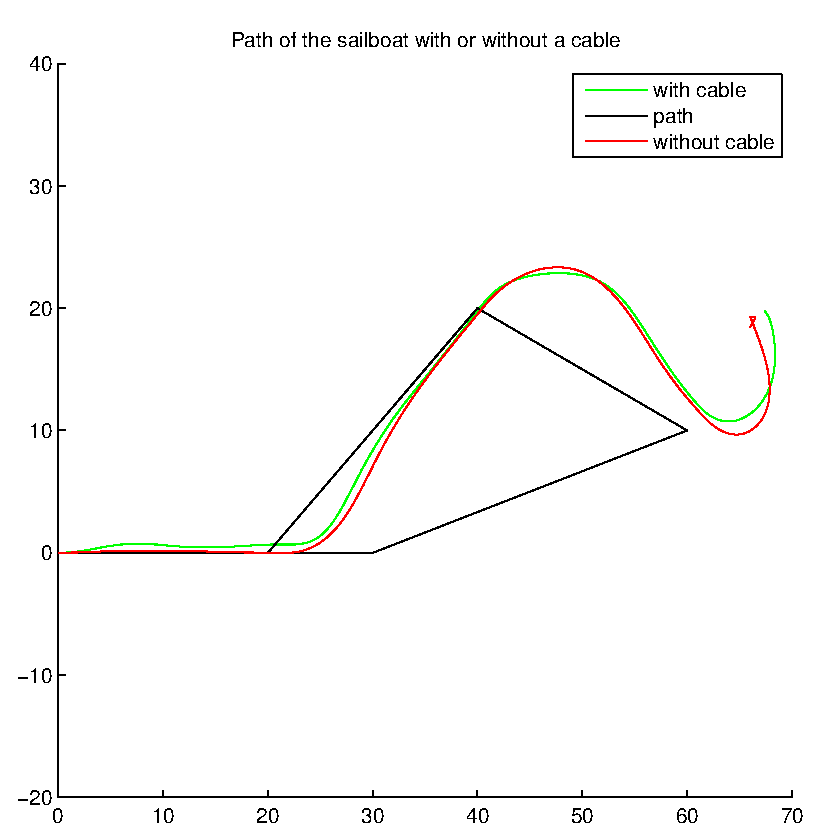
\includegraphics[scale=0.4,angle=0]{path_w_wtFig}
    \caption{Path taken by the boat with or without cable.}
    \label{fig:pathBoat}
\end{figure}

In figure~\ref{fig:pathBoat} the path of the boat with or without cable is represented, the boat is controlled each time by the algorithm from Le Bars and Jaulin 2013~\cite{LeBars2013}. The boat is less controllable in a straight
line, indeed the boat start at the position zero in the direction of the wind, the boat without cable follow very thoroughly the line but the boat with cable discard from the line.

The boat with cable look more efficient when turning but it would be because of the lesser speed.



\chapter{Viability of the model}
To test the model, a cable with a pressure sensor has been put on the boat in order to capture the behaviour
of the cable.

First the gathered data will be compared with the old model for tuning. Then the test with cable will be compared to the new model.

Different test has been realised to test the boat:

\begin{itemize}
\item salut
\item re
\end{itemize}

\chapter{Simulator}
\section{Simulator for the C++ program}

To help and create a faster development for the Sailing Robot project the creation of a simulator would be useful, in the testing of the \gls{C++} program used to control the boat. 
There is some simulator to test the algorithm and Matlab but the conversion from Matlab to C++ can induce some bugs that were not yet easy to identify.
The current design of the code at the time of the creation of the simulator was too complicated and old to be able to simply implement the simulation in the code itself, therefore the easiest way to do it was to pre-empt the connection to the sensor needed to drive the boat.

\begin{figure}[H]
\centering
\psscalebox{0.5 0.5} % Change this value to rescale the drawing.
{
% \usepackage[usenames,dvipsnames]{pstricks}
% \usepackage{epsfig}
% \usepackage{pst-grad} % For gradients
% \usepackage{pst-plot} % For axes
% \usepackage[space]{grffile} % For spaces in paths
% \usepackage{etoolbox} % For spaces in paths
% \makeatletter % For spaces in paths
% \patchcmd\Gread@eps{\@inputcheck#1 }{\@inputcheck"#1"\relax}{}{}
% \makeatother
% % User Packages:
% \usepackage{amsmath}
% \usepackage{amsfonts}
% \usepackage{amssymb}
% \usepackage{algorithm}
% \usepackage{algorithmic}
\psscalebox{1.0 1.0} % Change this value to rescale the drawing.
{
\begin{pspicture}(0,-4.398276)(16.057339,4.398276)
\definecolor{colour0}{rgb}{0.65882355,0.99607843,0.35686275}
\definecolor{colour1}{rgb}{0.42352942,0.8784314,0.9764706}
\definecolor{colour2}{rgb}{0.9490196,0.5764706,0.5921569}
\psellipse[linecolor=black, linewidth=0.012, linestyle=dashed, dash=0.17638889cm 0.10583334cm, dimen=outer](7.031034,-1.3086208)(3.0275862,2.689655)
\psellipse[linecolor=black, linewidth=0.04, fillstyle=solid,fillcolor=colour0, dimen=outer](1.854732,-1.6375979)(1.583172,0.8379661)
\rput{6.7314534}(0.37274778,-0.6346489){\psellipse[linecolor=black, linewidth=0.04, fillstyle=solid,fillcolor=colour1, dimen=outer](5.5820684,2.8517241)(4.02,1.03)}
\rput{18.753927}(0.70229614,-3.9860935){\psellipse[linecolor=black, linewidth=0.04, fillstyle=solid,fillcolor=colour2, dimen=outer](12.42028,0.13337229)(1.8921099,2.7825892)}
\psline[linecolor=black, linewidth=0.04, arrowsize=0.05291667cm 2.0,arrowlength=1.4,arrowinset=0.0]{<->}(13.57026,-2.8102677)(13.243397,-1.9115297)
\rput[bl](11.606252,-3.1447155){Remote PC Control}
\rput[bl](12.480103,-1.7166519){Xbee}
\psline[linecolor=black, linewidth=0.04, arrowsize=0.05291667cm 2.0,arrowlength=1.4,arrowinset=0.0]{<->}(12.382069,-1.649387)(8.717011,-1.7143679)
\rput[bl](0.0,-2.964253){\textbf{TCP/IP Communication}}
\rput[bl](0.67349714,-1.7868472){WebServer}
\psline[linecolor=black, linewidth=0.04, arrowsize=0.05291667cm 2.0,arrowlength=1.4,arrowinset=0.0]{<->}(2.6210194,-1.6705922)(5.202069,-1.6582758)
\rput[bl](4.0903444,4.1182756){\textbf{I$^2$C Communication}}
\rput[bl](11.2173395,2.923399){\textbf{Serial Port Communication}}
\rput[bl](3.1420686,2.6217241){Pressure Sensor}
\psline[linecolor=black, linewidth=0.04, arrowsize=0.05291667cm 2.0,arrowlength=1.4,arrowinset=0.0]{->}(3.8220687,2.221724)(5.8420687,-0.17827587)
\rput[bl](11.319171,-0.44599622){Motor Controllor}
\psline[linecolor=black, linewidth=0.04, arrowsize=0.05291667cm 2.0,arrowlength=1.4,arrowinset=0.0]{<->}(11.245878,-0.48970443)(8.711275,-1.4573234)
\rput[bl](11.18373,0.52905947){Windsensor}
\psline[linecolor=black, linewidth=0.04, arrowsize=0.05291667cm 2.0,arrowlength=1.4,arrowinset=0.0]{->}(11.224926,0.5702956)(8.577307,-0.78335524)
\rput[bl](7.4620686,3.0017242){Compass}
\psline[linecolor=black, linewidth=0.04, arrowsize=0.05291667cm 2.0,arrowlength=1.4,arrowinset=0.0]{->}(7.5820684,2.7417243)(7.3420687,0.24172413)
\rput[bl](11.263345,1.9251283){GPS}
\psline[linecolor=black, linewidth=0.04, arrowsize=0.05291667cm 2.0,arrowlength=1.4,arrowinset=0.0]{->}(11.182069,1.9017241)(9.023218,0.5121456)
\rput[bl](5.8620687,-1.6782758){Main Program}
\pscircle[linecolor=black, linewidth=0.04, dimen=outer](6.9620686,-1.5382758){1.78}
\rput[bl](7.382758,-4.398276){\textit{Computing Unit}}
\psline[linecolor=black, linewidth=0.04, arrowsize=0.05291667cm 2.0,arrowlength=1.4,arrowinset=0.0]{->}(8.676984,0.12884279)(8.280845,-0.39293915)
\rput[bl](7.965766,0.2254468){{\small GPSD Daemon}}
\end{pspicture}
}


}
\caption{Data transfer model of the boat.}
\label{fig:model_boat_}
\end{figure}

As seen on~\ref{fig:model_boat_}, the data goes from and to the main program regulating the boat via three different mean of communication.
The sensor data comes from serial ports \gls{RS232} and \gls{i2c} communication and the program send data to the remote web server via \gls{TCPIP}. The simulator only need to deal with two of the communication path, \gls{i2c} and serial communication, as the web server will always be available. 

\gls{linux} allow to create easily many virtual serial ports via programming but it is no possible to do the same for \gls{i2c} communication. To remediate at this problem the solution is to bypass function used by the main program to discuss with the I$^2$C bus. The program use a dynamic library (not compiled inside the program  and loaded in memory at runtime), functions can be overloaded if other functions with the same prototype (same name, same input parameters and same output) are loaded before. Then those function will communicate with the exterior of the program  with \gls{sharedmemory}.

\begin{figure}[H]
\centering
\psscalebox{0.5 0.5} % Change this value to rescale the drawing.
{
% \usepackage[usenames,dvipsnames]{pstricks}
% \usepackage{epsfig}
% \usepackage{pst-grad} % For gradients
% \usepackage{pst-plot} % For axes
% \usepackage[space]{grffile} % For spaces in paths
% \usepackage{etoolbox} % For spaces in paths
% \makeatletter % For spaces in paths
% \patchcmd\Gread@eps{\@inputcheck#1 }{\@inputcheck"#1"\relax}{}{}
% \makeatother
% % User Packages:
% \usepackage{amsmath}
% \usepackage{amsfonts}
% \usepackage{amssymb}
% \usepackage{algorithm}
% \usepackage{algorithmic}
\psscalebox{1.0 1.0} % Change this value to rescale the drawing.
{
\begin{pspicture}(0,-4.3745584)(16.869757,4.3745584)
\definecolor{colour0}{rgb}{0.99607843,0.16470589,0.16470589}
\definecolor{colour5}{rgb}{0.99607843,0.99607843,0.99607843}
\definecolor{colour1}{rgb}{0.65882355,0.99607843,0.35686275}
\definecolor{colour2}{rgb}{0.9490196,0.5764706,0.5921569}
\definecolor{colour3}{rgb}{0.79607844,0.7607843,0.24705882}
\definecolor{colour4}{rgb}{0.6627451,0.25490198,0.63529414}
\psellipse[linecolor=black, linewidth=0.04, fillstyle=vlines, hatchwidth=0.02, hatchangle=22.0, hatchsep=0.4, hatchcolor=colour0, dimen=outer](8.260985,2.9066384)(1.6181818,1.2121212)
\psframe[linecolor=colour5, linewidth=0.04, fillstyle=solid,fillcolor=colour5, dimen=outer](9.34314,3.2042816)(7.0468435,2.4931705)
\rput{-33.63478}(1.1742575,4.476236){\psellipse[linecolor=black, linewidth=0.012, linestyle=dashed, dash=0.17638889cm 0.10583334cm, dimen=outer](7.99201,0.29558465)(3.9300253,4.396972)}
\rput{-330.17743}(-0.2676209,-1.0106432){\psellipse[linecolor=black, linewidth=0.04, fillstyle=solid,fillcolor=colour1, dimen=outer](1.7638229,-1.0078198)(1.5165052,1.3591782)}
\rput{18.753927}(0.18432017,-4.216627){\psellipse[linecolor=black, linewidth=0.04, fillstyle=solid,fillcolor=colour2, dimen=outer](12.859304,-1.5502272)(1.0433294,0.39234522)}
\psline[linecolor=black, linewidth=0.04, arrowsize=0.05291667cm 2.0,arrowlength=1.4,arrowinset=0.0]{<->}(13.57026,-2.7865503)(13.243397,-1.8878121)
\rput[bl](11.606252,-3.120998){Remote PC Control}
\rput[bl](12.480103,-1.6929344){Xbee}
\psline[linecolor=black, linewidth=0.04, arrowsize=0.05291667cm 2.0,arrowlength=1.4,arrowinset=0.0]{<->}(12.382069,-1.6256695)(8.717011,-1.6906502)
\rput[bl](0.0,-2.9405355){\textbf{TCP/IP Communication}}
\rput[bl](0.67349714,-1.7631297){WebServer}
\psline[linecolor=black, linewidth=0.04, arrowsize=0.05291667cm 2.0,arrowlength=1.4,arrowinset=0.0]{<->}(2.6210194,-1.6468747)(5.202069,-1.6345583)
\rput[bl](12.029757,-0.96005267){\textbf{Serial Port Communication}}
\rput[bl](5.7583647,-1.7138176){Main Program}
\pscircle[linecolor=black, linewidth=0.04, dimen=outer](6.9620686,-1.5145583){1.78}
\rput[bl](7.382758,-4.3745584){\textit{Computing Unit}}
\psline[linecolor=black, linewidth=0.04, arrowsize=0.05291667cm 2.0,arrowlength=1.4,arrowinset=0.0]{->}(8.676984,0.15256032)(8.280845,-0.3692216)
\rput[bl](7.965766,0.24916434){{\small GPSD Daemon}}
\psline[linecolor=colour3, linewidth=0.04, linestyle=dashed, dash=0.17638889cm 0.10583334cm, arrowsize=0.05291667cm 2.0,arrowlength=1.4,arrowinset=0.0]{->}(9.624621,2.203608)(11.345834,0.5793657)(8.570076,-0.7782101)
\psline[linecolor=colour3, linewidth=0.04, linestyle=dashed, dash=0.17638889cm 0.10583334cm, arrowsize=0.05291667cm 2.0,arrowlength=1.4,arrowinset=0.0]{<->}(8.667046,-0.9963919)(11.903409,0.5793657)(9.806439,2.6036081)
\psline[linecolor=colour3, linewidth=0.04, linestyle=dashed, dash=0.17638889cm 0.10583334cm, arrowsize=0.05291667cm 2.0,arrowlength=1.4,arrowinset=0.0]{->}(8.630682,1.7308809)(8.71553,0.61572933)
\rput[bl](1.1640154,-0.4024525){Simulator}
\psline[linecolor=black, linewidth=0.04, arrowsize=0.05291667cm 2.0,arrowlength=1.4,arrowinset=0.0]{<->}(6.679167,2.7005777)(1.7943184,0.082395986)
\rput{-44.561977}(1.2363315,7.8739686){\rput[bl](10.226605,2.428315){\small{Motor Controller}}}
\rput{-41.194386}(1.1743914,6.7127047){\rput[bl](9.517955,1.7939111){\small{Windsensor}}}
\rput{-85.93802}(6.6179576,10.209451){\rput[bl](8.789066,1.5524297){\small{GPS}}}
\rput{77.81638}(5.4495893,-6.1740537){\rput[bl](6.54947,0.28886062){\scriptsize{Pressure Sensor}}}
\rput{76.49165}(6.109742,-6.8746214){\rput[bl](7.415733,0.43835557){\small{Compass}}}
\psline[linecolor=colour4, linewidth=0.06, linestyle=dotted, dotsep=0.10583334cm, arrowsize=0.05291667cm 2.0,arrowlength=1.4,arrowinset=0.0]{->}(7.2157326,2.2028)(6.672029,-0.2105333)
\psline[linecolor=colour4, linewidth=0.06, linestyle=dotted, dotsep=0.10583334cm, arrowsize=0.05291667cm 2.0,arrowlength=1.4,arrowinset=0.0]{->}(7.8335104,1.9583555)(7.279436,-0.32016295)
\psline[linecolor=colour4, linewidth=0.06, linestyle=dotted, dotsep=0.10583334cm, arrowsize=0.05291667cm 2.0,arrowlength=1.4,arrowinset=0.0]{->}(16.157822,1.8314756)(12.598345,1.8346128)
\psline[linecolor=colour3, linewidth=0.04, linestyle=dashed, dash=0.17638889cm 0.10583334cm, arrowsize=0.05291667cm 2.0,arrowlength=1.4,arrowinset=0.0]{->}(16.090996,3.0593288)(12.557545,3.0620859)
\rput[bl](13.239436,3.2190964){Virtual Serial Port}
\rput[bl](13.491288,1.9450222){Shared Memory}
\rput[bl](7.216541,2.6736417){Side Program}
\psellipse[linecolor=black, linewidth=0.04, fillstyle=vlines, hatchwidth=0.02, hatchangle=22.0, hatchsep=0.4, hatchcolor=colour0, dimen=outer](7.0246215,-0.16608886)(0.7777778,0.36296296)
\end{pspicture}
}


}
\caption{Data transfer model of the boat with simulator.}
\label{fig:model_boat_sim}
\end{figure}

The implementation of the simulator need a program on the same computing unit as the main program to be able to use virtual serial ports and \gls{sharedmemory}, this side program is used as a proxy for the simulator, the communication is via \gls{TCPIP} to allow easy configuration (i.e.\ changing parameters of the simulation on a computer and the main program running on the embedded computer allowing to test the code directly on the computer that will be sailing).
The data transferred between the simulator and the side program are raw values, the side program will 
then transform the data for serial port as the real sensor messages, e.g.\ \gls{NMEA} messages for the GPS and 
wind sensor.

The main program was then refactor to a node and message program, meaning each sensor is a node sending messages to the node that will compute the orders to give to the actuators. The program created before work without changes on this model, but to follow the model of the program a simulation as been created , the node directly send the messages inside the program and is still discussing with the simulator with \gls{TCPIP}.
The advantage of this simulation is a simpler initialisation but the first implementation still as some advantage such as allowing testing different preprocessing of data (filters).

In the end this simulator is useful as it help the programmer testing quickly the code and the implementation of the algorithm without doing real test.


\section{Work method}

\section{Smith predictor}

The sailboat have many thing that will delay the effect of the control,
reason is the lag generated by the time taken by the actuators to take their positions




\chapter{Miscellaneous}

\section{Work method}

\section{Smith predictor}

The sailboat have many thing that will delay the effect of the control,
reason is the lag generated by the time taken by the actuators to take their positions
%\addcontentsline{toc}{part}{Conclusion}
%----------------------------------------------------------------------------------------
%\appendix
\chapter*{Appendix 1}
\addcontentsline{toc}{chapter}{Appendix 1}
%simulation cable longer
\chapter*{Appendix 2}
\addcontentsline{toc}{chapter}{Appendix 2}
%use matlab
\chapter*{Appendix 3}
\addcontentsline{toc}{chapter}{Appendix 3}
%use simulator get the info data


%----------------------------------------------------------------------------------------
%	BIBLIOGRAPHIE
%----------------------------------------------------------------------------------------
%\addcontentsline{toc}{part}{Bibliography}
%\bibliographystyle{apalike-fr}
\bibliographystyle{IEEEtran}
\bibliography{bibliographie}
\addcontentsline{toc}{part}{Bibliography}
\nocite{*}


%----------------------------------------------------------------------------------------

\end{document}